\section{Introduction}

Hopfield Networks were invented by John Hopfield in 1982 under the name of \textit{associative neural network}. They are content addressable binary memory systems that are used to model associative memory problems: 
\begin{quote}
\textit{Store a set of $p$ patterns $\psi_i^\mu$ in such a way that when presented with a new pattern $\zeta_i$, the network responds by producing whichever one of the stored patterns most closely resembles $\zeta_i$} \citep{Polk:2002fk}
\end{quote}

\begin{wrapfigure}{r}{6cm}
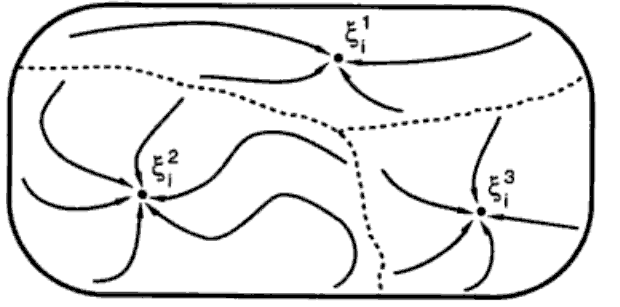
\includegraphics[width=6cm,angle=0]{PatternAttractors.png}
\caption{Configuration space showing the patterns as attractors}
\label{fig:PatternAttractors}
\end{wrapfigure}

In the configuration space of the network, the stored patterns $\psi_i^\mu$ act as attractors. While a Hopfield network is guaranteed to converge to a local minimum, convergence to one of the stored patterns is not a necessity. 

In order to facilitate the mathematical computation, the basis of the binary system is changed from a $\{0,1\}$ base to a $\{-1,1\}$ base.

